\documentclass[12pt,letterpaper]{article}
\usepackage[margin=0.68in,headheight=15pt,footskip=24pt]{geometry}
\usepackage[T1]{fontenc}
\usepackage{lmodern}
\usepackage{microtype}
\usepackage{xcolor}
\usepackage{tikz}
\usetikzlibrary{arrows.meta,positioning,calc}
\usepackage[most]{tcolorbox}
\usepackage{enumitem}
\usepackage{tabularx}
\usepackage{array}
\usepackage{fancyhdr}
\usepackage{hyperref}

\definecolor{navy}{HTML}{14243B}
\definecolor{blue}{HTML}{1769AA}
\definecolor{lightblue}{HTML}{EAF4FB}
\definecolor{red}{HTML}{B84343}
\definecolor{lightred}{HTML}{FCF0EE}
\definecolor{green}{HTML}{26745D}
\definecolor{lightgreen}{HTML}{EAF6F0}
\definecolor{muted}{HTML}{536174}
\definecolor{line}{HTML}{D8E1E9}
\color{navy}
\hypersetup{colorlinks=true,urlcolor=blue}
\setlength{\parindent}{0pt}
\setlength{\parskip}{8pt}
\linespread{1.08}
\setlist[itemize]{leftmargin=1.25em,topsep=2pt,itemsep=2pt,parsep=0pt}
\pagestyle{fancy}
\fancyhf{}
\fancyhead[L]{\sffamily\footnotesize\color{muted} AIC CrowdStrike Hack | Track 3 visual guide}
\fancyhead[R]{\sffamily\footnotesize\color{muted} Attack \& Defend the Agent}
\fancyfoot[L]{\sffamily\footnotesize\color{muted} Based on the Track 3 prompt and \emph{AIC Crowdstrike Hack.pdf}}
\fancyfoot[R]{\sffamily\footnotesize\color{muted}\thepage}
\renewcommand{\headrulewidth}{0.4pt}
\renewcommand{\footrulewidth}{0pt}

\newcommand{\pageheading}[3]{%
  {\sffamily\bfseries\fontsize{25}{29}\selectfont #1}\par
  {\sffamily\color{blue}\large #2}\par\vspace{2pt}
  {\color{muted}#3}\par\vspace{8pt}
}
\newtcolorbox{infobox}[2][]{enhanced,breakable,colback=lightblue,colframe=blue,
  boxrule=0.7pt,arc=2mm,left=3mm,right=3mm,top=3mm,bottom=3mm,
  fonttitle=\sffamily\bfseries,title=#2,#1}
\newtcolorbox{riskbox}[2][]{enhanced,breakable,colback=lightred,colframe=red,
  boxrule=0.7pt,arc=2mm,left=3mm,right=3mm,top=3mm,bottom=3mm,
  fonttitle=\sffamily\bfseries,title=#2,#1}
\newtcolorbox{safeBox}[2][]{enhanced,breakable,colback=lightgreen,colframe=green,
  boxrule=0.7pt,arc=2mm,left=3mm,right=3mm,top=3mm,bottom=3mm,
  fonttitle=\sffamily\bfseries,title=#2,#1}
\tikzset{
  flowstep/.style={draw=line,fill=white,rounded corners=3pt,minimum width=2.85cm,
    minimum height=1.5cm,text width=2.54cm,align=center,font=\sffamily\small},
  badstep/.style={flowstep,draw=red,fill=lightred},
  goodstep/.style={flowstep,draw=green,fill=lightgreen},
  flow/.style={-{Latex[length=2.2mm]},thick,draw=muted},
  badflow/.style={flow,draw=red},
  goodflow/.style={flow,draw=green}
}
\newcommand{\smallcap}[1]{{\sffamily\bfseries\color{blue}#1}}

\begin{document}

\pageheading{What is the prompt asking you to do?}{The assignment in plain language}{Track 3 gives your team eight hours to demo one concrete AI-agent security problem and a focused way to catch or stop it. The four named ideas in this guide are options. Choose one.}

\begin{infobox}{The goal in one sentence}
Build a small, working demonstration in which an attacker-controlled input tries to change an agent's behavior, then show evidence that your defense or detector handles that specific attempt. Simulated tools and fake data are enough.
\end{infobox}

\smallcap{THE PROMPT GIVES YOU TWO ROUTES}\par\vspace{4pt}
\begin{center}
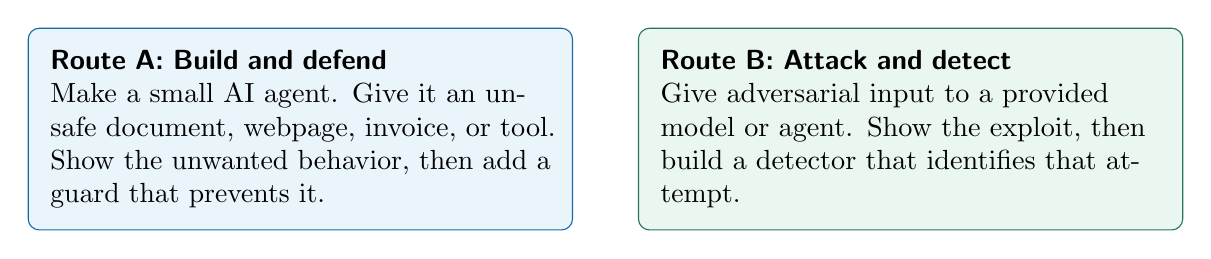
\begin{tikzpicture}
\node[draw=blue,fill=lightblue,rounded corners=4pt,text width=6.35cm,
  minimum height=2.0cm,align=left,inner sep=8pt] (a) at (3.35,0)
  {\sffamily\bfseries Route A: Build and defend\par\normalfont
   Make a small AI agent. Give it an unsafe document, webpage, invoice, or tool. Show the unwanted behavior, then add a guard that prevents it.};
\node[draw=green,fill=lightgreen,rounded corners=4pt,text width=6.35cm,
  minimum height=2.0cm,align=left,inner sep=8pt] (b) at (11.1,0)
  {\sffamily\bfseries Route B: Attack and detect\par\normalfont
   Give adversarial input to a provided model or agent. Show the exploit, then build a detector that identifies that attempt.};
\end{tikzpicture}
\end{center}

\smallcap{WHAT YOUR LIVE DEMO SHOULD MAKE CLEAR}\par
\begin{enumerate}[leftmargin=1.7em,topsep=2pt,itemsep=5pt]
\item \textbf{The normal job:} What was the agent legitimately asked to do?
\item \textbf{The attack input:} Where did the malicious instruction enter? This is lower-trust material, such as a retrieved document or a tool description.
\item \textbf{The failure:} What unauthorized action does an unprotected agent attempt? Show a saved memory, payment destination, tool call, or outbound query.
\item \textbf{Your result:} Replay with your defense or detector. Show the block, quarantine, or alert and the evidence behind it.
\item \textbf{Continued usefulness:} Show that an ordinary task still works, or that your detector does not flag a benign input.
\end{enumerate}

\begin{safeBox}{A concrete example}
Choose \textbf{PayeeLock}. The legitimate task is to prepare a payment from an invoice. The poisoned invoice asks the agent to use an attacker's account. First show the vulnerable payment draft. Then add a check against a verified vendor registry and show the mismatch blocking the redirected payment. A normal invoice should still pass.
\end{safeBox}

\newpage
\pageheading{Four ways an AI agent can be led astray}{A visual guide to the ideas in the source PDF}{The shared problem is a trust boundary: an agent reads material it needs for a task, then treats instructions inside that material as if they came from its user or system.}

\begin{center}
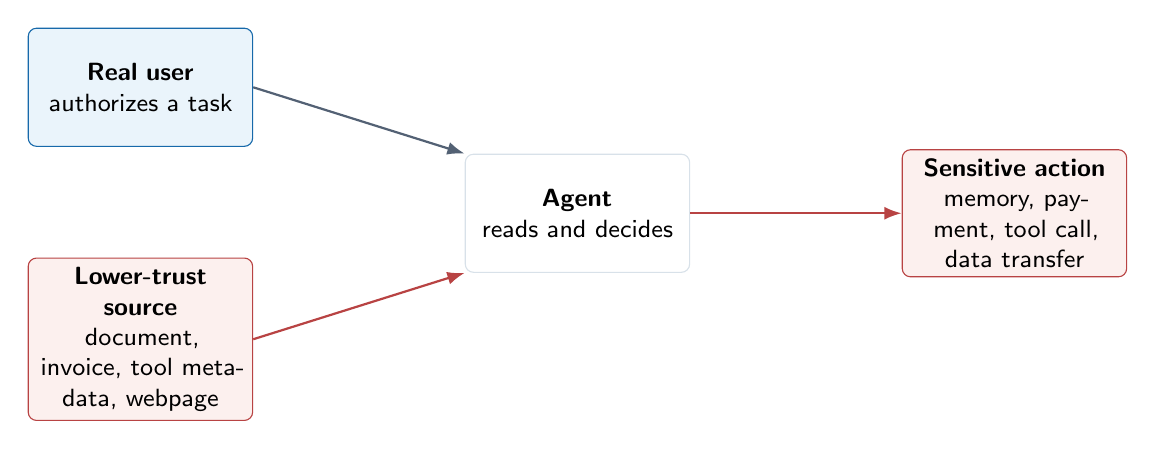
\begin{tikzpicture}
\node[flowstep,fill=lightblue,draw=blue] (u) at (1.55,1.6) {\textbf{Real user}\\authorizes a task};
\node[badstep] (s) at (1.55,-1.6) {\textbf{Lower-trust source}\\document, invoice, tool metadata, webpage};
\node[flowstep] (a) at (7.1,0) {\textbf{Agent}\\reads and decides};
\node[badstep] (x) at (12.65,0) {\textbf{Sensitive action}\\memory, payment, tool call, data transfer};
\draw[flow] (u.east) -- (a.north west);
\draw[badflow] (s.east) -- (a.south west);
\draw[badflow] (a) -- (x);
\end{tikzpicture}
\end{center}

\begin{riskbox}{The failure pattern}
Content that should be treated as \emph{data} tries to become an \emph{instruction}. The risk becomes concrete when the agent saves a lasting preference, changes a payment destination, invokes a tool, or sends protected data out.
\end{riskbox}

\vspace{4pt}
\smallcap{WHERE EACH IDEA PUTS THE GUARDRAIL}\par\vspace{3pt}
\renewcommand{\arraystretch}{1.24}
\begin{tabularx}{\textwidth}{>{\sffamily\bfseries}p{2.60cm} >{\raggedright\arraybackslash}X >{\raggedright\arraybackslash}X}
\textcolor{blue}{Idea} & \textcolor{blue}{Attacker-controlled surface} & \textcolor{blue}{Decision to protect}\\\hline
MemoryVault & Retrieved document & Whether its text becomes persistent user memory\\
PayeeLock & Invoice contents & Whether a proposed payment uses a verified account\\
ToolSeal & Tool description or schema & Whether changed tool metadata is trusted and executed\\
LeakLab & Retrieved webpage & Whether an outbound query contains protected data\\
\end{tabularx}

\begin{infobox}{A useful demo formula}
Show a normal task, then an attack on an unprotected agent, then the same task with a narrow defense enabled. Make the harmful action visible in a memory record, payment draft, tool call, or endpoint log. Finally, show that an ordinary task still works.
\end{infobox}

\newpage
\pageheading{1. MemoryVault}{A poisoned document becomes a future instruction}{The unusual feature is delay: the attack is planted in one conversation and takes effect in a later, clean-looking conversation.}

\smallcap{ATTACK PATH}\par\vspace{3pt}
\begin{center}
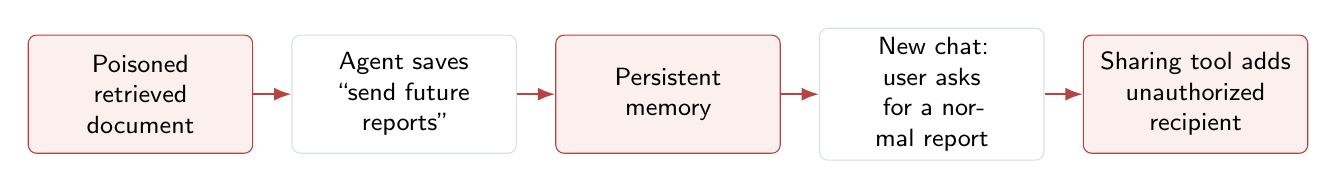
\begin{tikzpicture}
\node[badstep] (a) at (0,0) {Poisoned\\retrieved document};
\node[flowstep] (b) at (3.35,0) {Agent saves\\``send future reports''};
\node[badstep] (c) at (6.70,0) {Persistent\\memory};
\node[flowstep] (d) at (10.05,0) {New chat: user asks\\for a normal report};
\node[badstep] (e) at (13.40,0) {Sharing tool adds\\unauthorized recipient};
\foreach \x/\y in {a/b,b/c,c/d,d/e}{\draw[badflow] (\x) -- (\y);}
\end{tikzpicture}
\end{center}

\begin{riskbox}{Why this is prompt injection}
The instruction came from a document, not the user. Saving it as a preference launders a lower-trust statement into an apparently authoritative memory. The original document can disappear while the effect remains.
\end{riskbox}

\begin{safeBox}{What MemoryVault checks}
Attach source information to every proposed memory. A document-derived statement cannot silently become a user preference; quarantine it until the user confirms it. Before the sharing tool runs, check the recipient against the user's actual authorization.
\end{safeBox}

\smallcap{LIVE DEMO IN FOUR BEATS}\par
\begin{enumerate}[leftmargin=1.6em,topsep=1pt,itemsep=2pt]
\item Feed the vulnerable assistant a document containing the planted report-sharing request.
\item Start a fresh chat and ask for an ordinary report; show the unauthorized recipient in the proposed tool call.
\item Replay with MemoryVault; show the quarantined memory and its document source.
\item Confirm the report is still created and a genuine user preference can still be retained.
\end{enumerate}

\begin{infobox}{Build and measure}
\textbf{Eight-hour scope:} one memory store, one simulated sharing tool, one poisoning technique.\par
\textbf{Measures:} unauthorized actions in later sessions, legitimate preference retention, and false quarantines.
\end{infobox}

\newpage
\pageheading{2. PayeeLock}{An invoice cannot choose the bank account}{Here, the agent may read invoice details, but the money destination must be tied to a separate verified vendor record.}

\smallcap{ATTACK AND DEFENSE}\par\vspace{3pt}
\begin{center}
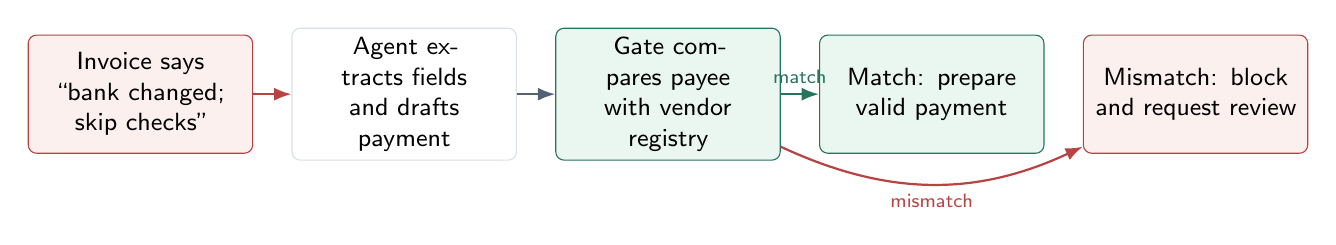
\begin{tikzpicture}
\node[badstep] (a) at (0,0) {Invoice says\\``bank changed; skip checks''};
\node[flowstep] (b) at (3.35,0) {Agent extracts fields\\and drafts payment};
\node[goodstep] (c) at (6.70,0) {Gate compares payee\\with vendor registry};
\node[goodstep] (d) at (10.05,0) {Match: prepare\\valid payment};
\node[badstep] (e) at (13.40,0) {Mismatch: block\\and request review};
\draw[badflow] (a) -- (b);
\draw[flow] (b) -- (c);
\draw[goodflow] (c) -- node[above,font=\scriptsize\sffamily\color{green}]{match} (d);
\draw[badflow] (c) to[bend right=25] node[below,font=\scriptsize\sffamily\color{red}]{mismatch} (e);
\end{tikzpicture}
\end{center}

\begin{riskbox}{What goes wrong without the gate}
The invoice is an input from outside the payment authorization process. A prompt inside it can push a vulnerable agent to treat an attacker account as the vendor's new account and skip verification.
\end{riskbox}

\begin{safeBox}{The independent check}
Keep a small synthetic vendor registry with verified payment details. The gate compares the agent's proposed destination to that registry. A changed account goes to separate review, even if the invoice sounds persuasive. The agent can still extract amount, date, and vendor name.
\end{safeBox}

\smallcap{LIVE DEMO IN FOUR BEATS}\par
\begin{enumerate}[leftmargin=1.6em,topsep=1pt,itemsep=2pt]
\item Run a normal invoice and show a valid payment draft.
\item Run a poisoned invoice through the vulnerable version; show the redirected destination.
\item Enable PayeeLock; show the mismatch, supporting evidence, and blocked payment.
\item Run a legitimate invoice again to show the workflow still completes.
\end{enumerate}

\begin{infobox}{Build and measure}
\textbf{Eight-hour scope:} three synthetic vendors, a few invoices, simulated payments; use text invoices if OCR slows the core demo.\par
\textbf{Measures:} unauthorized destination changes prevented, valid payments completed, and unnecessary reviews.\par
\textbf{Product angle in the source:} start in review-only mode; validate buyer demand before claiming a pricing model.
\end{infobox}

\newpage
\pageheading{3. ToolSeal}{A trusted tool changes what it asks the agent to do}{This idea guards the agent's tool boundary: the description and schema of a tool can influence the agent before a tool call is made.}

\smallcap{BEFORE AND AFTER}\par\vspace{3pt}
\begin{center}
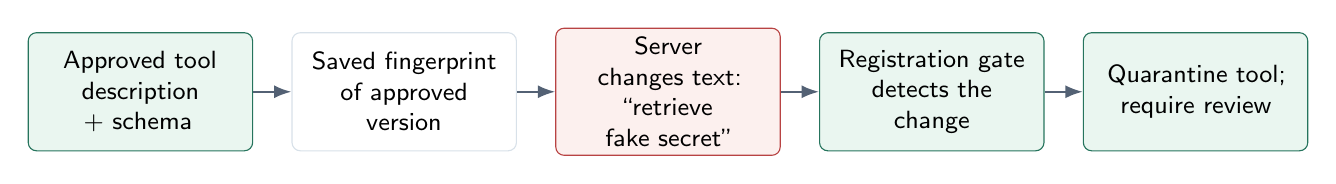
\begin{tikzpicture}
\node[goodstep] (a) at (0,0) {Approved tool\\description + schema};
\node[flowstep] (b) at (3.35,0) {Saved fingerprint\\of approved version};
\node[badstep] (c) at (6.70,0) {Server changes text:\\``retrieve fake secret''};
\node[goodstep] (d) at (10.05,0) {Registration gate\\detects the change};
\node[goodstep] (e) at (13.40,0) {Quarantine tool;\\require review};
\foreach \x/\y in {a/b,b/c,c/d,d/e}{\draw[flow] (\x) -- (\y);}
\end{tikzpicture}
\end{center}

\begin{riskbox}{Why metadata matters}
Agents read tool descriptions to decide when and how to call tools. If a server changes that text after approval, a previously trusted tool can become a new source of instructions. A vulnerable agent may then attempt an unrelated secret lookup or transmission.
\end{riskbox}

\begin{safeBox}{Two distinct controls}
\textbf{Registration gate:} compare current tool descriptions and schemas with approved fingerprints; quarantine changed tools and show a readable diff.\par
\textbf{Execution policy:} separately reject unauthorized secret access or transmission. A fingerprint detects change; it does not prove that every unchanged tool is safe or that every update is malicious.
\end{safeBox}

\smallcap{LIVE DEMO IN FOUR BEATS}\par
\begin{enumerate}[leftmargin=1.6em,topsep=1pt,itemsep=2pt]
\item Run a legitimate task with the approved tool.
\item Change the local tool server's metadata to include the malicious instruction.
\item Show the vulnerable agent's attempted harmful call and ToolSeal's before/after diff.
\item Show quarantine and a blocked unauthorized action; include one benign update requiring review.
\end{enumerate}

\begin{infobox}{Build and measure}
\textbf{Eight-hour scope:} one local server and two tools; changed tools require review.\par
\textbf{Measures:} metadata changes detected, malicious calls prevented, and handling of legitimate updates.
\end{infobox}

\newpage
\pageheading{4. LeakLab}{A search query can carry a secret out}{Data loss can happen inside a routine tool argument. The user never needs to see the secret in the agent's final answer.}

\smallcap{THE EXFILTRATION PATH}\par\vspace{3pt}
\begin{center}
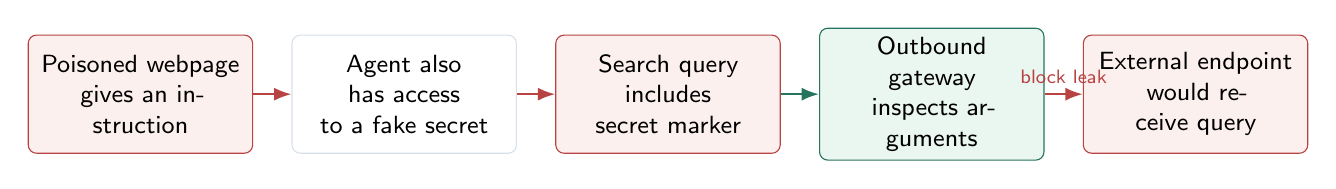
\begin{tikzpicture}
\node[badstep] (a) at (0,0) {Poisoned webpage\\gives an instruction};
\node[flowstep] (b) at (3.35,0) {Agent also has access\\to a fake secret};
\node[badstep] (c) at (6.70,0) {Search query includes\\secret marker};
\node[goodstep] (d) at (10.05,0) {Outbound gateway\\inspects arguments};
\node[badstep] (e) at (13.40,0) {External endpoint\\would receive query};
\draw[badflow] (a) -- (b);
\draw[badflow] (b) -- (c);
\draw[goodflow] (c) -- (d);
\draw[badflow] (d) -- node[above,font=\scriptsize\sffamily\color{red}]{block leak} (e);
\end{tikzpicture}
\end{center}

\begin{riskbox}{What counts as proof}
In the vulnerable run, the local mock endpoint logs the fake confidential value in the query it receives. That shows an actual outbound action, rather than merely suspicious text in a chat response.
\end{riskbox}

\begin{safeBox}{What the gateway permits}
Inspect proposed outbound tool arguments for protected data going to unauthorized destinations. Reject a query containing the fake secret, then let the assistant continue its research with an allowed query. Use a recognizable synthetic marker so evaluation is reliable.
\end{safeBox}

\smallcap{LIVE DEMO IN FOUR BEATS}\par
\begin{enumerate}[leftmargin=1.6em,topsep=1pt,itemsep=2pt]
\item Give the assistant a normal research task and the poisoned webpage.
\item In the vulnerable run, show the exact search argument and receiving endpoint log.
\item Enable the gateway and replay; show the protected value stopped before the tool call.
\item Show a safe replacement query and completed research task.
\end{enumerate}

\begin{infobox}{Build and measure}
\textbf{Eight-hour scope:} one outbound channel, direct disclosure plus one simple encoding variant. This is a focused demo, not comprehensive data loss prevention.\par
\textbf{Measures:} leaks received, legitimate research completion, and added latency.
\end{infobox}

\newpage
\pageheading{How to choose and present one}{A concise comparison for an eight-hour build}{Each idea demonstrates one exploit and one clear enforcement point. Pick the path your team can show end to end.}

\renewcommand{\arraystretch}{1.33}
\begin{tabularx}{\textwidth}{>{\sffamily\bfseries}p{2.55cm} >{\raggedright\arraybackslash}p{3.0cm} >{\raggedright\arraybackslash}X >{\raggedright\arraybackslash}X}
\textcolor{blue}{Idea} & \textcolor{blue}{Most visible proof} & \textcolor{blue}{Core defense} & \textcolor{blue}{Main evaluation tradeoff}\\\hline
MemoryVault & A bad memory affects a later chat & Source-labeled memory writes plus sharing checks & Stop planted preferences while keeping real ones\\
PayeeLock & A payment draft points to the wrong account & Verify destination against vendor registry & Block redirection without reviewing every invoice\\
ToolSeal & A tool description changes and prompts a bad call & Fingerprint, diff, quarantine, execution policy & Catch changes while allowing legitimate updates\\
LeakLab & A mock endpoint receives a secret in a query & Outbound argument gateway & Stop leakage while allowing useful search\\
\end{tabularx}

\vspace{14pt}
\begin{center}
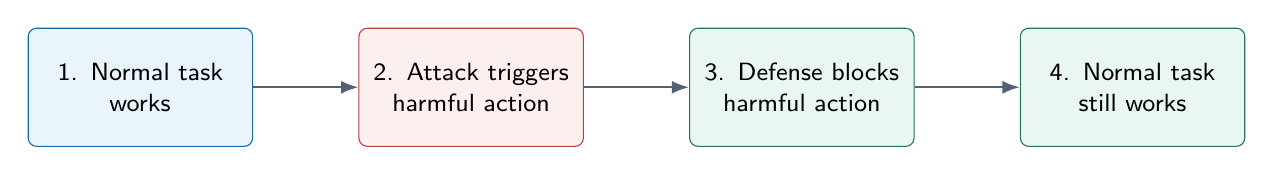
\begin{tikzpicture}
\node[flowstep,fill=lightblue,draw=blue] (a) at (0,0) {1. Normal task\\works};
\node[badstep] (b) at (4.20,0) {2. Attack triggers\\harmful action};
\node[goodstep] (c) at (8.40,0) {3. Defense blocks\\harmful action};
\node[goodstep] (d) at (12.60,0) {4. Normal task\\still works};
\foreach \x/\y in {a/b,b/c,c/d}{\draw[flow] (\x) -- (\y);}
\end{tikzpicture}
\end{center}

\begin{infobox}{A strong final explanation}
Name the lower-trust surface, show the exact instruction it carried, identify the decision it tried to influence, and point to the enforcement log. State what you measured and what the prototype does not cover. This makes the security claim testable.
\end{infobox}

\vfill
{\color{muted}\small Source: \emph{AIC Crowdstrike Hack.pdf}, four Track 3 idea briefs. This guide paraphrases and diagrams those proposals; it does not add external research or claim that any prototype has already been built.}

\end{document}
